\documentclass{beamer}
\usepackage{../common_slides}
\usepackage{tikz}
\usepackage{tikz-qtree}
\usepackage{pdfpages}

\title{Course Review and AlphaGo}
\date{}
\author{CS 287}

\begin{document}
\begin{frame}
  \titlepage
\end{frame}


\begin{frame}{Today's Lecture}
  \begin{itemize}
  \item Overview of the models/tasks covered course
    \air
    \air 
  \item AlphaGo 
  \end{itemize}
\end{frame}

\section{Course Review}

\begin{frame}{Foundational Challenge: Turing Test}
  \begin{quote}
    Q: Please write me a sonnet on the subject of the Forth Bridge.

    A : Count me out on this one. I never could write poetry.

    Q: Add 34957 to 70764.
    
    A: (Pause about 30 seconds and then give as answer) 105621.
    
    Q: Do you play chess?
    
    A: Yes.
    
    Q: I have K at my K1, and no other pieces. You have only K at K6 and R at R1. It is your move. What do you play?

    A: (After a pause of 15 seconds) R-R8 mate.
      {\normalfont - Turing (1950)}
  \end{quote}

\end{frame}

\begin{frame}{(1) Lexicons and Lexical Semantics}
  \textbf{Zipf' Law (1935,1949):}
  \begin{quote}
    The frequency of any word is inversely proportional to its rank in the frequency table.
  \end{quote}


     \begin{center}
       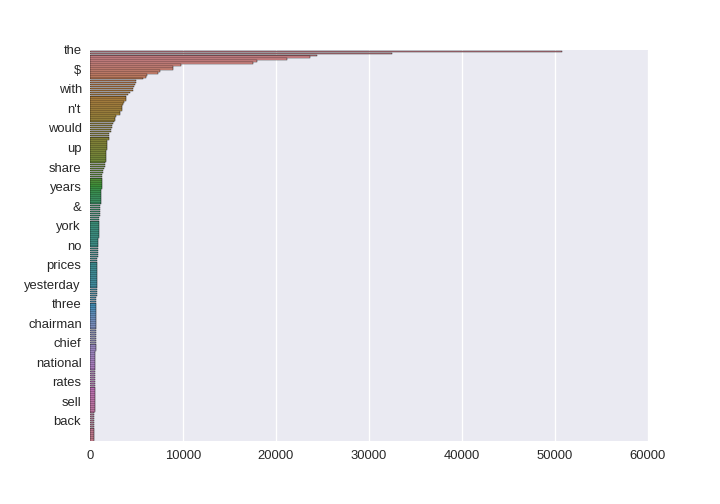
\includegraphics[width=0.8\textwidth]{../notebooks/zipf}         
     \end{center}
% \begin{itemize}
  % \item I.e. it is common to use rare words. 
  % \item Central issue in NLP is dealing cleverly with rare words. 
  % \end{itemize}
\end{frame}


\begin{frame}{(2) Structure and Probabilistic Modeling }
  \textbf{The Shannon Game (Shannon and Weaver, 1949):}
  \begin{quote}
    Given the last $n$ words, can we predict the next one?
  \end{quote} 
  

  \texttt{The pin-tailed snipe (Gallinago stenura) is a small stocky wader. It breeds in northern Russia and migrates to spend the \_\_ } 


  \begin{itemize}
  \item Probabilistic models have become very effective at this task.
  \item Crucial for speech recognition (Jelinek), OCR, automatic translations, etc. 
  \end{itemize}



\end{frame}

\begin{frame}{(3) Compositionality of Syntax and Semantics}
  \begin{quote}
    Probabilistic models give no insight into some of the basic
    problems of syntactic structure  {\normalfont - Chomsky (1956)}
  \end{quote}
  \begin{center}
    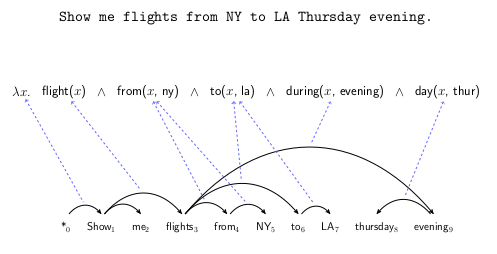
\includegraphics[width=10cm]{syntaxsem}
  \end{center}
\end{frame}


\begin{frame}{(4) Document Structure and Discourse}
  \begin{quote}
    Language is not merely a bag-of-words but a tool with particular
    properties  { - \normalfont Harris (1954)}
  \end{quote}
  \begin{center}
    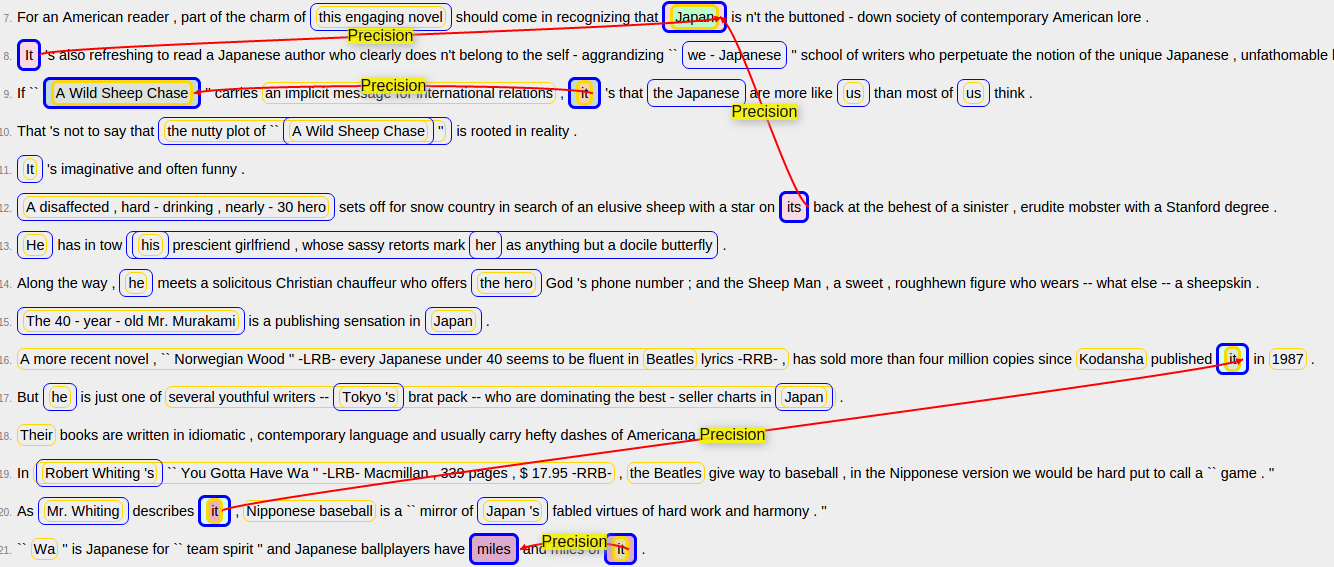
\includegraphics[width=\textwidth]{cort}
  \end{center}
\end{frame}

\begin{frame}{(5) Knowledge and Reasoning Beyond the Text}
\begin{quote}
It is based on the belief that in modeling language understanding, we must deal in an integrated way with all of the aspects of language — syntax, semantics, and inference. {- \normalfont Winograd (1972) }  
\end{quote}


\texttt{The city councilmen refused the demonstrators a permit because they [feared/advocated] violence.}


\begin{itemize}
\item Recently (2011) posed as a challenge for testing commonsense reasoning.  

\end{itemize}
\end{frame}


\section{Modeling}



\begin{frame}{Machine Learning Approaches to NLP}
  
  Many problem-specific modeling questions,
  \begin{itemize}
  \item $\boldx$; input representation
  \item $\boldy$; output representation 
  \item Model architecture
  \item Objective
  \end{itemize}
  \air 

  \textbf{This Course:} Focus on supervised data-driven, end-to-end approaches
\end{frame}

\begin{frame}{Input Representations}
  \begin{enumerate}
  \item Sparse Features
  \item Dense Features (Embeddings)
  \item Convolutional NN
  \item Recurrent NN
  \end{enumerate}
\end{frame}

{
\setbeamercolor{background canvas}{bg=}
\includepdf[pages=3-8]{slides_wpi.pdf}
}

{
\setbeamercolor{background canvas}{bg=}
\includepdf[pages=10-14]{slides_wpi.pdf}
}


\begin{frame}{What model should I use?}
  Questions to ask: 
  \begin{itemize}
  \item Do I have significant amounts of supervised data?
  \item Do I have prior knowledge of my problem/domain?
  \item What is the underlying metric of interest?
  \item Do I need interpretability of the model? 
  \item Is the structure of the text important?
  \item Is training efficiency/prediction efficiency important?
  \end{itemize}
\end{frame}


\begin{frame}[fragile]{Example: Simple Question Answering}
\begin{verbatim}
  10 Mary moved to the hallway.
  11 Daniel travelled to the office.
  12 Where is Daniel?     office  11
\end{verbatim}

  \begin{itemize}
  \item Input is the sentences and the question
    \air 
  \item Output is a set of possible answers.
    \air 
  \item How might you go about selecting an answer?
  \end{itemize}

\end{frame}




% \begin{frame}{}
%   ``Count-based Models''
%   \begin{itemize}
%   \item Naive Bayes, Kneser-Ney LM, HMM, 
%   \end{itemize}

%   \pause

%   \begin{itemize}
%   \item \structure{Fast to train, convex}
%   \item \structure{Interpretable}
%   \item \alert{Quite sensitive to features/independence assumptions}
%   \item \alert{Need smoothing, overfitting hacks}
%   \end{itemize}
% \end{frame}

% \begin{frame}
%   Discriminative Linear models
%   \air 

%   \begin{itemize}
%   \item Multiclass LR, windowed features, MEMM
%   \end{itemize}
%   \pause
  
%   \begin{itemize}
%   \item \structure{Convex}
%   \item \structure{Somewhat interpretable}
%   \item \alert{Sensitive to feature choice}
%   \item \alert{Requires optimization to train}
%   \end{itemize}
% \end{frame}


% \begin{frame}{Sparse Feature Approach}
%   \begin{itemize}
%   \item $p(y) p(x|y)$
%   \end{itemize}
%   \begin{itemize}
%   \item $p(y)$ prior on answers
%   \item $p(x|y)$ determined by feature set.  
%   \end{itemize}
% \end{frame}

% \begin{frame}[fragile]{Pipeline Sparse Feature Approach}

% \begin{verbatim}
%   11 [Daniel] travelled to the [office].
%   12 Where is [Daniel]?     office  11
% \end{verbatim}

%   \begin{enumerate}
%   \item Run tagging to POS tags.
%   \item Run NER to find named entities.
%   \item Run parsing to find syntax.
%   \item Construct Features from this data i.e. 
%     Mary  
    
%   \end{enumerate}
% \end{frame}

% \begin{frame}{Stanford CoreNLP}
  
% \end{frame}


% \begin{frame}
%   Shallow feed-forward neural networks
%   \air 

%   \begin{itemize}
%   \item Windowed NN, CBoW Embeddings, Bengio NNLM, NN-MEMM
%   \end{itemize}
%   \pause

%   \begin{itemize}
%   \item \structure{Learn feature combinations end-to-end}
%   \item \structure{Improved performance on several tasks}
%   \item \alert{Non-convex}
%   \item \alert{Requires large amount of (semi-)supervision}
%   \item \alert{Sensitive to hyper-parameters}
%   \end{itemize}
% \end{frame}

% \begin{frame}[fragile]{End-to-End Simple Approach}

% \begin{verbatim}
%   11 [Daniel] travelled to the [office].
%   12 Where is [Daniel]?     office  11
% \end{verbatim}

%   \begin{enumerate}
%   \item Use CBoW or convolution to construct word representation 
%   \item Use  
%   \item Train end-to-end
%   \end{enumerate}
% \end{frame}


% \begin{frame}
%   Recurrent neural networks
%   \begin{itemize}
%   \item RNN/GRU/LSTM, acceptor, transducer, encoder-decoder
%   \end{itemize}

%   \begin{itemize}
%   \item \structure{Learn feature combinations end-to-end}
%   \item \structure{Learn sequence representation (!) end-to-end}
%   \item \structure{Improved performance of sequence modeling tasks}
%   \item \alert{Non-convex, and sensitive to exploding/vanishing gradient}
%   \item \alert{Requires large amount of (semi-)supervision}
%   \item \alert{Sensitive to training, hyper-parameters, model size}
%   \item Requires greedy/beam search (non-Markovian)
%   \end{itemize}
% \end{frame}

% \begin{frame}[fragile]
% \begin{verbatim}
%   11 [Daniel] travelled to the [office].
%   12 Where is [Daniel]?     office  11
% \end{verbatim}

%   \begin{enumerate}
%   \item Use RNN to construct representation
%   \item Train end-to-end
%   \end{enumerate}
% \end{frame}


% \begin{frame}{Loss Functions}
%   \begin{itemize}
%   \item Generative $p(x, y)$
%     \begin{itemize}
%     \item Maximum Likelihood
%     \item Smoothing
%     \end{itemize}
%   \item Discriminative $p(y | x)$
%     \begin{itemize}
%     \item Cross-Entropy 
%      \item Hinge Loss
%     \end{itemize}
%   \end{itemize}
% \end{frame}


% {
% \setbeamercolor{background canvas}{bg=}
% \includepdf[pages=19]{slides_wpi.pdf}
% }

% \begin{frame}{Output Representations}
%   \begin{enumerate}
%   \item Ranking (score the output)
%   \item Simple Multiclass Output
%   \item Large Multiclass Output (HSM, NCE) 
%   \item Structured (sequence)
%   \end{enumerate}
% \end{frame}


% \begin{frame}{Search}
%   \begin{enumerate}
%   \item Multiclass Prediction
%   \item Greedy Search
%   \item Beam Search
%   \item Viterbi Search
%   \end{enumerate}
% \end{frame}

% \begin{frame}{Tasks}
%   \begin{itemize}
%   \item Text Classification 
%   \item Part-of-Speech Tagging
%   \item Language Modeling
%   \item Sequence Modeling
%   \item Named-Entity Recognition
%   \end{itemize}
% \end{frame}

\section{AlphaGo}


\begin{frame}
  \begin{center}
    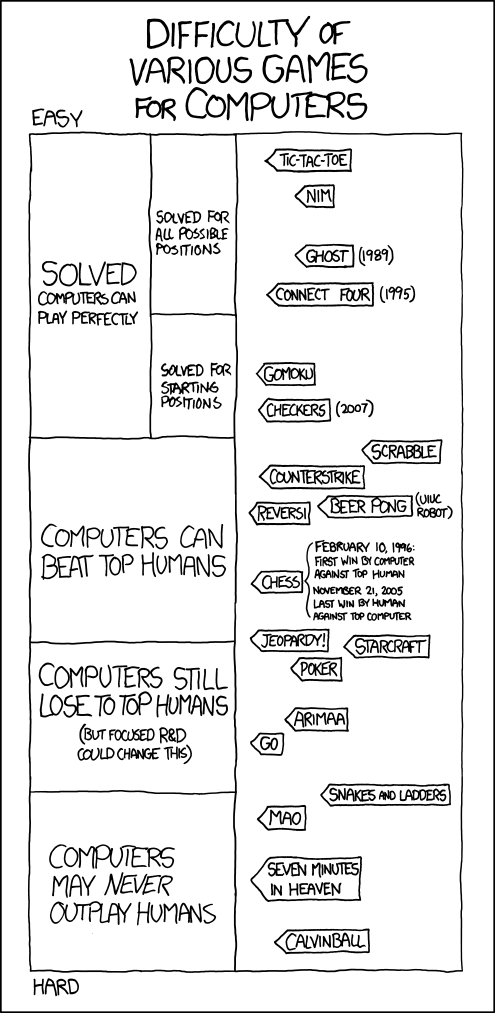
\includegraphics[height=\textheight]{gameais}
  \end{center}
\end{frame}

\begin{frame}
  \url{https://www.youtube.com/watch?v=Jq5SObMdV3o}
\end{frame}

\begin{frame}{}
  \begin{center}
    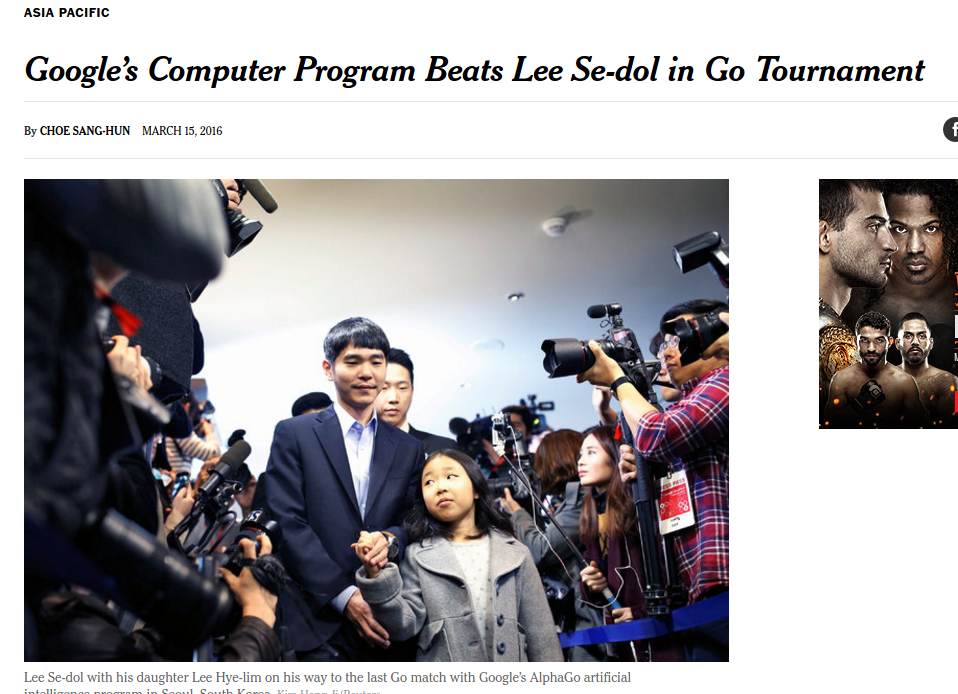
\includegraphics[width=\textwidth]{alphago/nyt}
  \end{center}
\end{frame}

\begin{frame}{AlphaGo Overview}

  \begin{enumerate}
  \item Learn a model to predict one-step move from experts
    \air 
  \item Refine by self-play reinforcement learning
    \air
  \item Use as part of game-tree search.
  \end{enumerate}
\end{frame}

\begin{frame}{Policy Setup}
  Given current board state $s$, distribution over actions $a$. 

  \begin{itemize}
  \item Learn a policy, $p(a | s)$ 
    \air 
  \item Estimate distribution with softmax.
    \air 
  \item Gives a one-step Go player. 
  \end{itemize}
\end{frame}

\begin{frame}{(1) Policy Network}
  Learned from 29.4 million positions from 160,000 expert games

  Two models:
  \begin{itemize}
  \item $p_{\pi}(a | s)$; multiclass logistic regression (pattern+sparse features)
  \item $p_{\sigma}(a | s)$; deep convolutional network
  \end{itemize}

  \begin{center}
    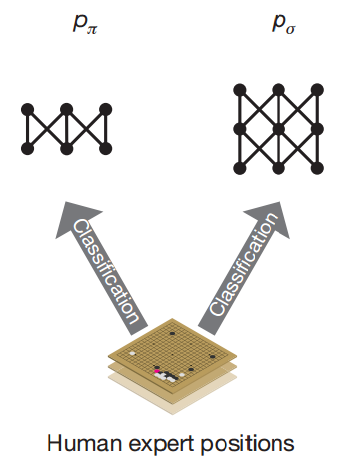
\includegraphics[width=5cm]{alphago/sup}
  \end{center}

\end{frame}


% \begin{frame}{Go Windowed Model}
%   \begin{itemize}
%   \item Represent board by 5x5 Squares
%     \air
%   \item Raw board is input to the network 
%   \end{itemize}
% \end{frame}

\begin{frame}
  \begin{center}
    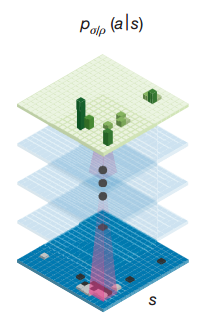
\includegraphics[width=5cm]{alphago/deepconv}
  \end{center}
  % \begin{itemize}
  % \item 13 conv layers
  % \item ReLU nonlinearities
  % \end{itemize}
\end{frame}



\begin{frame}{Deep Convolutional Network}
  \begin{quote}
    The first hidden layer zero pads the input into a 23x23 image, then convolves k filters of kernel size 5x5 with stride
1 with the input image and applies a rectifier nonlinearity. Each of the subsequent
hidden layers 2 to 12 zero pads the respective previous hidden layer into a 21x21
image, then convolves k filters of kernel size 3×3 with stride 1, again followed
by a rectifier nonlinearity. 
  \end{quote}
\end{frame}

\begin{frame}{Deep Convolutional Network}
  \begin{quote}
    The first hidden layer zero pads the input into a 23x23 image, then convolves k filters of kernel size 5x5 with stride
1 with the input image and applies a rectifier nonlinearity. Each of the subsequent
hidden layers 2 to 12 zero pads the respective previous hidden layer into a 21x21
image, then convolves k filters of kernel size 3×3 with stride 1, again followed
by a rectifier nonlinearity. 
  \end{quote}
\end{frame}


\begin{frame}
  \begin{quote}
     The step size $\alpha$ was initialized to 0.003 and was halved
every 80 million training steps, without momentum terms, and a mini-batch size
of $m=16$. Updates were applied asynchronously on 50 GPUs using DistBelief 61;
gradients older than 100 steps were discarded. Training took around 3 weeks for
340 million training steps.
  \end{quote}
\end{frame}


\begin{frame}{(2) Reinforcement Learning}


  \begin{itemize}
  \item Refine one-step player by playing against itself. 
    \air 
  \item Popular technique for stochastic games (TD-Gammon)
    \air
  \item Reinforcement learning objects to account for single-step bias
  \end{itemize}
\end{frame}


\begin{frame}{Self-Play with Policy Gradient}
  Start with $p_{\sigma}$ and play against itself to learn:

  \begin{itemize}
  \item  $p_{\rho}(a | s)$; deep convolution network (policy gradient)
  \end{itemize}
  
  
  \textbf{Process:} Training epoch $J+1$ 
  \begin{enumerate}
  \item Sample opponent from previous version of model $j <J$
  \item Play game between players $p_{\rho^J}$ and $p_{\rho^j}$ 
  \item Update weights using policy gradient on RL objective
    \begin{center}
      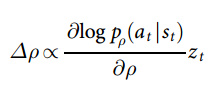
\includegraphics[width=5cm]{alphago/update}
    \end{center}
    where $z_t \in \{-1, 1\}$ represents the final outcome of the game.
  \end{enumerate}
\end{frame}

\begin{frame}{Value Network}
  \begin{itemize}
  \item Policy network trains only move at state.
  \item Useful also to know the value of a state. 
    \[ v(s) = E_{p_{\rho}}[z_t | s] \] 
  \end{itemize}
  \air 

  Generally done using game-specific heuristics.
\end{frame}

\begin{frame}{Value Network}
  Apply similar architecture for computing state value,

  \begin{itemize}
  \item $v_{\theta}$; deep CNN regression
    \air 
  \item Trained on self-play data set.
    \air 
  \item Minimize MSE with final self-play result.
  \end{itemize}
\end{frame}


\begin{frame}
  \begin{quote}
    When trained
on the KGS data set in this way, the value network memorized the
game outcomes rather than generalizing to new positions, achieving a
minimum MSE of 0.37 on the test set, compared to 0.19 on the training
set. To mitigate this problem, we generated a new self-play data set
consisting of 30 million distinct positions, each sampled from a separate
game. Each game was played between the RL policy network and
itself until the game terminated.
  \end{quote}
\end{frame}



% \begin{frame}
%   \begin{center}
%     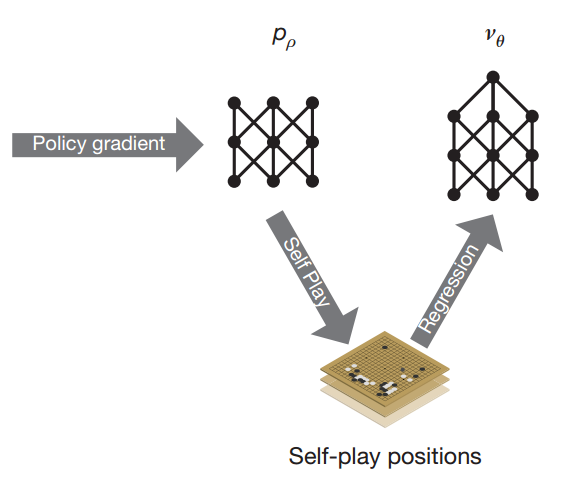
\includegraphics[width=0.8\textwidth]{alphago/policy}
%   \end{center}
% \end{frame}


\begin{frame}
  \begin{center}
    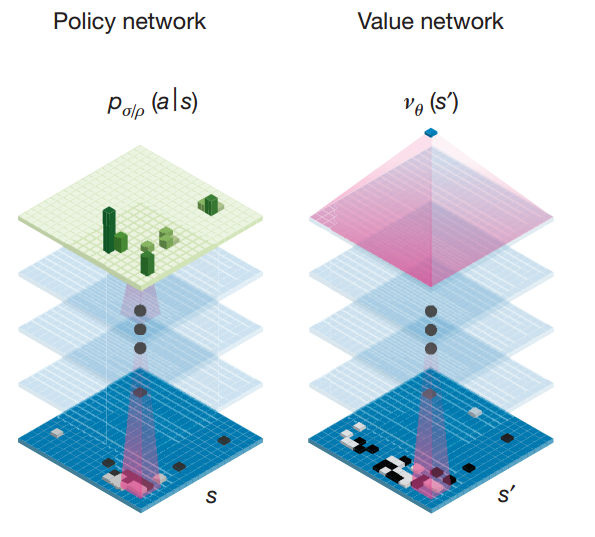
\includegraphics[width=0.8\textwidth]{alphago/conv}
  \end{center}
\end{frame}

\section{}

\begin{frame}
  \begin{center}
    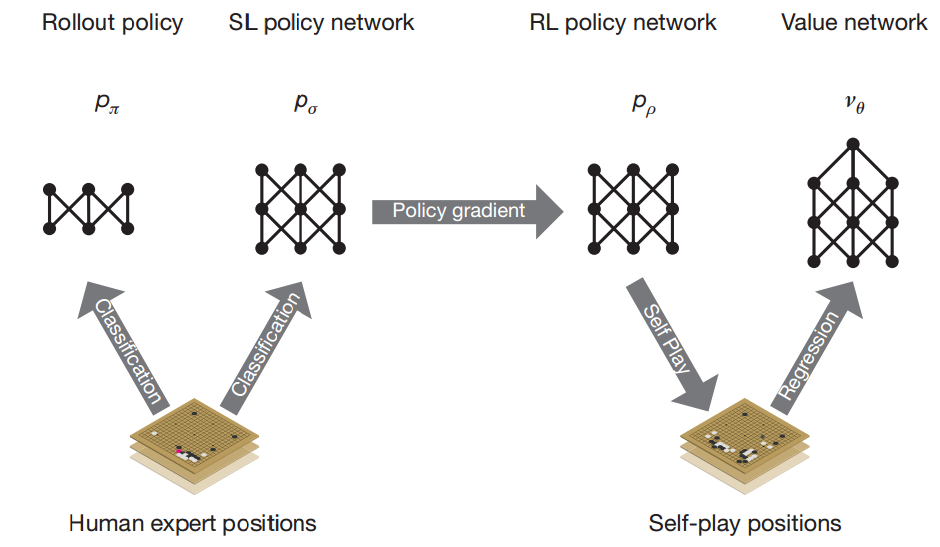
\includegraphics[width=\textwidth]{alphago/full}
  \end{center}
\end{frame}



\begin{frame}{(3) Game Search}
  Utilize the learned models with an advanced game-search algorithm
  \air 

  % \begin{center}
  %   \includegraphics[width=5cm]{tictactoe}
  % \end{center}
  \begin{itemize}
  \item Similar to standard game tree algorithms (CS182)
    \air 
  \item Monte Carlo Tree Search (MCTS)
    \begin{itemize}
    \item Select
    \item Expand
    \item Eval
    \item Update/Backup
    \end{itemize}
    \air
  \item Progressively expands the search space based on models
    
  \end{itemize}
\end{frame}


\begin{frame}{Select and Expansion}
  
  \begin{itemize}
  \item $Q(s,a)$; current expected value of taking action $a$ at $s$
    \air 
  \item $u(s, a)$; prior for taking $a$ at $s$ defined by $p_{\sigma}$   
  \end{itemize}

  \air 
  \textbf{Selection} step at state $s$,
  \[ \argmax_{a} Q(s,a) + u(s, a)\] 
  
  \air
  Based on selection, either move to seen node or \textbf{expand}.
\end{frame}

\begin{frame}{Game Search}
  \begin{center}
    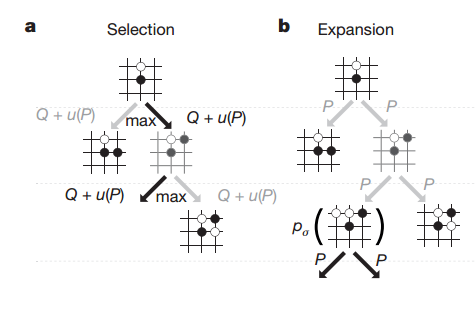
\includegraphics[width=\textwidth]{alphago/montecarlo}
  \end{center}
\end{frame}



% \begin{frame}
%   \begin{center}
%     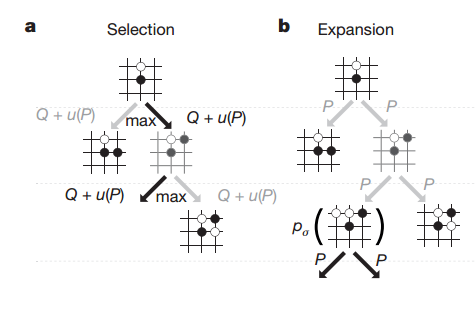
\includegraphics[width=\textwidth]{alphago/montecarlo}
%   \end{center}
% \end{frame}

\begin{frame}{State Evaluation}
  Reached ``leaf'' state $s_L$, want to \textbf{evaluate}

  \begin{itemize}
  \item Compute value as $V(s_L)$,
    \[ V(s_L) = (1-\lambda) v_\theta(s_l) + \lambda (R(s_L))\] 
   
    where $R$ is a rollout. Monte carlo simulation using $p_{\pi}$ 
    \air 
  \item Convex combination of value network and simulation under simple model
  \end{itemize}
  \air 

  Why not $p_{\sigma}$? Where did $p_{\rho}$ go?
\end{frame}

\begin{frame}
  \begin{center}
    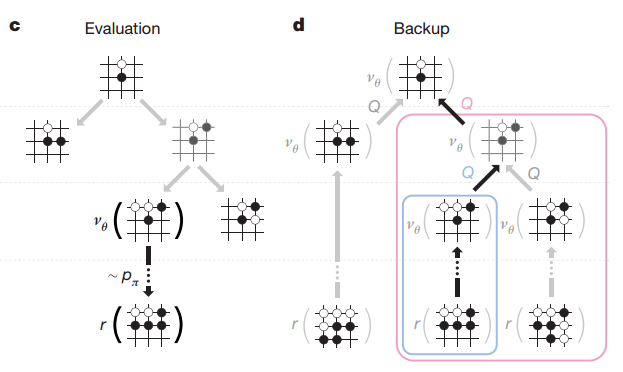
\includegraphics[width=\textwidth]{alphago/montecarlo2}
  \end{center}
\end{frame}

\begin{frame}{Move Selection}

  \begin{itemize}
  \item   After leaf evaluation all previous $Q$ values are 
    \textbf{updated} based on $V(s_L)$
    \air
  \item Process is run many times.
  \air
  \item Actual play is based on most commonly taken action. 
  \end{itemize}


\end{frame}


\begin{frame}{Results}
  \begin{center}
    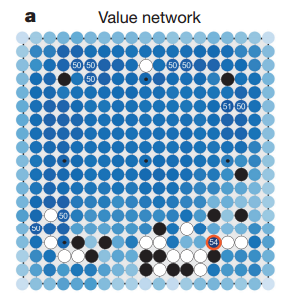
\includegraphics[height=\textheight]{alphago/vnet}
  \end{center}
\end{frame}

\begin{frame}{Results}
  \begin{center}
    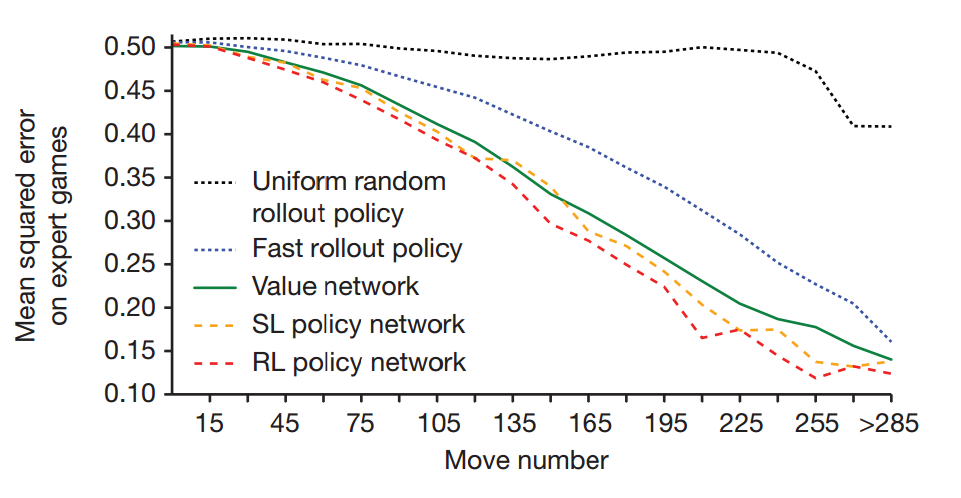
\includegraphics[width=\textwidth]{alphago/rollout}
  \end{center}
\end{frame}




\begin{frame}{Results}
  \begin{center}
    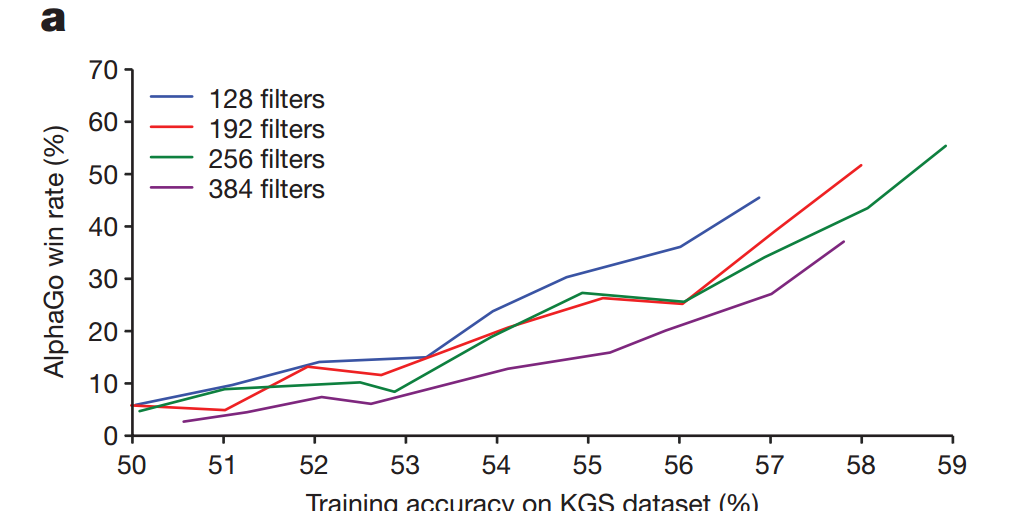
\includegraphics[width=\textwidth]{alphago/trainacc}
  \end{center}
\end{frame}

\begin{frame}{Results}
  \begin{center}
    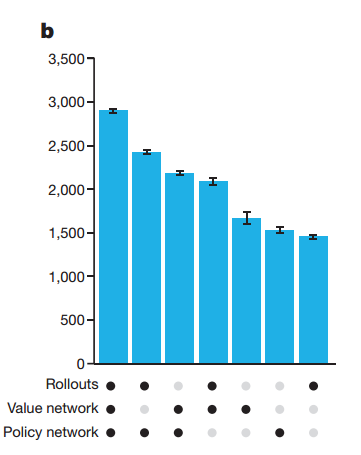
\includegraphics[width=5cm]{alphago/perf}
  \end{center}
\end{frame}


% \begin{frame}{Classical Tree Search}
  
% \end{frame}

% \begin{frame}{Depth-Limited Tree Search}
  
% \end{frame}


% \begin{frame}{Heuristic State Evaluation}
  
% \end{frame}

% \begin{frame}{Train on Data}
  
% \end{frame}


% \begin{frame}{Roll-Out}
  
% \end{frame}

% \begin{frame}{How do you compute this heuristic?}
  
% \end{frame}

% \begin{frame}{Learning Better Heuristic}
%   \begin{itemize}
%   \item Play game against itself
%   \item 
%   \end{itemize}
% \end{frame}

% \begin{frame}{Monte Carlo Tree Search}
  
% \end{frame}

% \begin{frame}
  
% \end{frame}

% \begin{frame}
  
% \end{frame}

\end{document}